\chapter{Dual Generator Offline Reinforcement Learning}




\newcommand{\name}{\text{DASCO}} 

Offline reinforcement learning (RL) algorithms aim to extract policies from datasets of previously logged experience. The promise of offline RL is to extract \textit{decision making engines} from existing data \cite{levine2020offline}. Such promise is especially appealing in domains where data collection is expensive or dangerous, but large amounts of data may already exists (e.g., robotics, autonomous driving, task-oriented dialog systems). Real-world datasets often consist of both expert and sub-optimal behaviors for the task of interest and also include potentially unrelated behavior corresponding to other tasks. While not all behaviors in the dataset are relevant for solving the task of interest, even sub-optimal trajectories can provide an RL algorithm with some useful information. In principle, if offline RL algorithms can combine segments of useful behavior spread across multiple sub-optimal trajectories together, the combined segments can then perform better than any behavior observed in the dataset. 

Effective offline RL requires estimating the value of actions other than those that were taken in the dataset, so as to pick actions that are better than the actions selected by the behavior policy. However, this requirement introduces a fundamental tension: the offline RL method must generalize to new actions, but it should not attempt to use actions in the Bellman backup for which the value simply cannot be estimated using the provided data. 
These are often referred to in the literature as out-of-distribution (OOD) actions~\cite{bear}. 
While a wide variety of methods have been proposed to constrain offline RL to avoid OOD actions~\cite{kostrikov2021offline, bcq, agarwal2019optimistic}, the formulation and enforcement of such constraints can be challenging, and might introduce considerable complexity, such as the need to explicitly estimate the behavior policy~\cite{brac} or evaluate high-dimensional integrals~\cite{kumar2020conservative}. Generative adversarial networks (GANs) in principle offer an appealing and simple solution: use the discriminator to estimate whether an action is in-distribution, and train the policy as the ``generator'' in the GAN formulation to fool this discriminator. Although some prior works have proposed variants on this approach~\cite{brac}, it has been proven difficult in practice as GANs can already suffer from instability when the discriminator is too powerful. Forcing the generator (i.e., the policy) to simultaneously \emph{both} maximize reward and fool the discriminator only exacerbates the issue of an overpowered discriminator.

We propose a novel solution that enables the effective use of GANs in offline RL, in the process not only mitigating the above challenge but also providing a more appealing form of support constraint that leads to improved performance. Our key observation is that the generative distribution in GANs can be split into \emph{two} separate distributions, one that represents the ``good parts'' of the data distribution and becomes the final learned policy, and an auxiliary generator that becomes the policy's complement, such that the mixture of the two is equal to the data distribution. This formulation removes the tension between maximizing rewards and matching the data distribution perfectly: as long as the learned policy is within the \emph{support} of the data distribution, the complement will pick up the slack and model the ``remainder" of the data distribution, allowing the two generators together to perfectly fool the discriminator. If however the policy ventures outside of the support of the data, the second generator cannot compensate for this mistake, and the discriminator will push the policy back inside the support. 
We name our method \name, for \textbf{D}ual-Generator \textbf{A}dversarial \textbf{S}upport \textbf{C}onstrained \textbf{O}ffline RL.

Experimentally, we demonstrate the benefits of our approach, \name{},
on standard benchmark tasks. For offline datasets that consist of a combination of expert, sub-optimal and noisy data,
our method outperforms distribution-constrained offline RL methods by a large margin.  


\section{Related Work}

Combining behaviors from sub-optimal trajectories to obtain high-performing policies is a central promise of offline RL. During offline training, querying the value function on unseen actions often leads to value over-estimation and unrecoverable collapse in learning progress. To avoid querying the value functions on out-of-distribution actions, existing methods encourage the learned policies to match the distribution of the dataset generation policies. This principle has been realized with a variety of practical algorithms ~\cite{jaques2019way,brac,peng2019awr,siegel2020keep,brac,kumar2019stabilizing, kostrikov2021offline,kostrikov2021offlineb,wang2020critic,fujimoto2021minimalist, BAIL, furuta2022generalized, jang2022gptcritic, meng2022offline, daoudi2022density, liu2022robust}.

For example, by optimizing the policies with respect to a conservative lower bound of the value function estimate \cite{kumar2020conservative}, only optimizing the policies on actions contained in the dataset \cite{kostrikov2021offline}, or jointly optimizing the policy on the long-term return and a behavior cloning objective \cite{fujimoto2021minimalist}. While \textit{explicitly} enforcing distribution constraint by adding the behavior cloning objective allows for good performance on near-optimal data, 
%the Gym locomotion tasks or on the D4RL benchmarks, 
this approach fails to produce good trajectories on sub-optimal datasets~\cite{kostrikov2021offline}.
%the antmaze-large and antmaze-medium tasks \cite{kostrikov2021offline}, which require stitching to obtain good performance \cite{d4rl}. 
Methods that \textit{implicitly} enforce distribution constraints, such as CQL and IQL, have seen more successes on such datasets.
%the antmaze-large and antmaze-medium tasks. 
However, they still struggle to produce near-optimal trajectories when the actions of the dataset generation policies are corrupted with noise or systematic biases (a result we demonstrate in Section~\ref{sec:exp}).
%%SL.5.18: The above discussion is reasonable, but it sets the expectation for the reader that the paper will demonstrate a significant improvement in terms of D4RL ant maze performance. If that's intended, then great. But if the results will be less amazing there, maybe revise this sentence a bit to set more realistic expectations?

However, enforcing distribution constraints  to avoid value over-estimation may not be necessary. It is sufficient to ensure the learned policies do not produce actions that are too unlikely under the dataset generation policy. That is, it is not necessary for the learned policy to fully \emph{cover} the data distribution, only to remain in-support~\cite{kumar2019stabilizing,kumar_blog,levine2020offline,brac,zhou2020plas,chen2022latent}. Unfortunately, previous methods that attempt to instantiate this principle into algorithms have not seen as much empirical success as algorithms that penalize the policies for not matching the action distribution of the behavior policies. In this paper, we propose a new GAN-based offline RL algorithm whose use of dual generators naturally induce support constraint and has competitive performance with recent offline RL methods. In a number of prior works, GANs have been used in the context of imitation learning to learn from expert data~\cite{gail,infogail,intentiongan,zhihanliu}. In this work, we show that dual-generator GANs can be used to learn from sub-optimal data in the context of offline RL.
% distribution constraint offline RL algorithms.
%%SL.5.18: Kind of a nitpick, but "distribution constraint offline RL algorithms" is very overloaded the way it is used, because it's debatable whether pessimism-based methods like CQL are really "distribution constraint" (for the purpose of this discussion, they actually are, but some readers might not understand this and object).
% What is especially puzzling is that existing support constraint offline RL algorithms do not perform as well as distribution constraint algorithms when learning from data sets that requires stitching, the scenario where we expect support constrained methods to clearly demonstrate their benefits. 
%%SL.5.18: While a valid point, this also sets an uncomfortable expectation that the paper will resolve this mystery (when in fact the paper doesn't do that, it just proposes a new method that works better). Maybe revise the above?

% TODO: add related work for GAN \textbf{GAN}

\section{Background}

Let $\mathcal{M} = (\mathcal{S}, \mathcal{A}, P, R, \gamma)$ define a Markov decision process (MDP), where $\mathcal{S}$ and $\mathcal{A}$ are state and action spaces, $P: \mathcal{S} \times \mathcal{A} \times \mathcal{S} \rightarrow \mathbb{R}_{+}$ is a state-transition probability function, $R: \mathcal{S} \times \mathcal{A} \rightarrow \mathbb{R}$ is a reward function and $\gamma$ is a discount factor. Reinforcement learning methods aim at finding a policy $\pi(a | s)$ that maximizes the expected discounted reward $R(\tau) = \sum_{t=0}^T \gamma^t R(s_t,a_t)$  over trajectories $\tau = (s_0, a_0, \dots, s_T, a_T)$ with time horizon $T$ induced by the policy $\pi$. 

In this work, we concentrate on the offline or off-policy RL setting, i.e. finding an optimal policy given a dataset $\mathcal{D}$ of previously collected experience $\tau \sim \mathcal{D}$ by a behavior policy $\pi_\beta$. A particularly popular family of methods for offline learning are based on training a Q-function through dynamic programming using temporal-difference (TD) learning~\cite{watkins1992q,sutton1998}. Such methods train a Q-function to satisfy the Bellman equation:
 \[
 Q (s_t, a_t) = R(s_t, a_t) + \gamma \mathbb{E}_{a\sim\pi} [Q(s_{t+1}, a)].
 \]
 $\pi(a | s) = \argmax_a Q_\theta(s,a)$
In Q-learning, the policy is replaced with a maximization, such that $\pi(a | s) = \argmax_a Q_\theta(s,a)$, while actor-critic methods optimize a separate parametric policy $\pi_\phi(a | s)$ that maximizes the Q-function. In this work, we extend the Soft Actor-Critic (SAC) method ~\cite{Haarnoja18} for learning from diverse offline datasets.

Generative Adversarial Networks (GANs)~\cite{GoodfellowPMXWOCB14} enable modeling a data distribution $p_{\mathcal{D}}$ through an adversarial game between a generator $G$ and a discriminator $D$:
% \begin{align}
%     \min_{\psi} \max_{\eta}  \mathbb{E}_{ x \sim p_{\mathcal{D}}} [\log(D_\eta(x))] + \mathbb{E}_{z \sim p(z)} [\log(1-D_\eta(G_\psi(z)))]
% \end{align}
\begin{align}
    \min_{G} \max_{D}  \mathbb{E}_{ x \sim p_{\mathcal{D}}} [\log(D(x))] + \mathbb{E}_{z \sim p(z)} [\log(1-D(G(z)))]
    \label{eq:vanilla_gan}
\end{align}

For this two player zero-sum game, \cite{GoodfellowPMXWOCB14} shows that for a fixed generator $G$, the optimal discriminator is $ D^*_G(x) = \dfrac{ p_{\mathcal{D} } (x) }{ p_{\mathcal{D} } (x) + p_{G }(x) }$ and the optimal generator matches the data distribution $ p^*_g(x) = p_{\mathcal{D}} $.

% The GAN framework has been used to model expert policy distributions through generative adversarial imitation learning (GAIL)~\cite{gail}. However, we note that GAIL 
%%SL.5.18: This is a bit of a red herring, since we are not actually building on GAIL (in fact, it might even be good to make it clear we are talking about GANs over *actions* not GAIL-style GANs over states)
GAN has been extended to the offline RL setting by interpreting the discriminator function as a measure of how likely an action is under the behavior policy, and jointly optimizing the policy to maximize an estimate of the long-term return and the discriminator function~\cite{brac}: 
\begin{align}
    \min_{\pi} \max_{D}  \mathbb{E}_{ s, a \sim p_{\mathcal{D}}} [\log(D(s,a))] + \mathbb{E}_{ s \sim p_{\mathcal{D}}, a \sim \pi(a|s) } [\log(1 - D(s,a))] - \mathbb{E}_{s \sim p_{\mathcal{D}}, a \sim \pi(a|s)} [ Q(s, a) ], \label{eq:brac}
\end{align}
%%SL.5.18: It feels like it might be a good idea to discuss the connection between this formulation and CQL, but I'm not sure where to do that -- it seems like it belongs more in related work, but it's probably a bit too technical for the related work section. Or maybe after we talk about how prior methods don't succeed, we can briefly remark that a latest approach (CQL) kind of does this but not exactly, and then say we'll compare to it?
where $Q(s,a)$ is trained via the Bellman operator to approximate the value function of the policy $\pi(a|s)$.
%Our algorithm is an actor-critic method, which alternates between policy evaluation and improvement steps. We begin the description of our algorithm by first introduc the objective functions that have been used in prior works. Since we study the offline RL problem, both the policy evaluation and improvement steps are performed using states from the offline dataset. 
This leads to iterative policy evaluation and policy improvement rules for the actor and the policy~\cite{brac}. During the $k^{th}$ update step, given the most recent values for the policy $\pi^{k}$, the value function $Q^{k}$, and the discriminator $D^k$, we perform the following updates to obtain the next values for the value function and the policy:
\begin{align}
\begin{split}
\label{eq:brac_update}
    Q^{k+1} \leftarrow& \argmin_{Q} \E_{s, a, s' \sim \mathcal{D}}\left[ \left((R(s, a) +  \gamma \E_{a' \sim {\policy}^k(a'|s')}[Q^{k}(s', a')]) - Q_{target}(s, a)\right)^2 \right]\\ 
    \policy^{k+1} \leftarrow& \argmax_{\policy} \E_{s \sim \mathcal{D}, a \sim \policy^k(a|s)}\left[Q^{k+1}(s, a) + \log D^k(s,a) \right]
\end{split}
\end{align}
where the $\log D(a|s)$ term in the policy objective aims at regularizing the learnt policy to prevent it from outputting OOD actions. In practice, training the policy to maximize both the value function and discriminator might lead to conflicting objectives for the policy and thus poor performance on either objective.
This can happen when the data contains a mixture of good and bad actions. Maximizing the value function would mean avoiding low-reward behaviors. On the other hand, maximizing the discriminator would require outputting all in-distribution actions, including sub-optimal ones. Our approach alleviates this conflict and enables \textit{in support} maximization of the value function when learning from mixed-quality datasets.

%he addition of $\log D(\ba|\bs)$ to the policy objective is often referred as policy regularization, in contrast to adding $\log D(\ba|\bs)$ to the value function target.


% Although aimed at enabling in-support optimization of the policy,
%%SL.5.18: the above (standard GAN) is not actually trying to do support, it's just a standard (JSD) distribution constraint
% in practice, maximizing both the Q-values and discriminator scores leads to conflicting objectives for the policy $\pi$ and often to unstable training.
%%SL.5.18: will this statement come across as controversial? maybe it's ok, but it kind of just seems to be asserted without evidence



\section{Dual-Generator Adversarial Support Constraint Offline RL}

We now present our algorithm, which uses a novel dual-generator GAN in combination with a weighting method to enable GAN-based offline RL that constrains the learned policy to remain within the support of the data distribution. We call our method \textit{Dual-generator Adversarial Support Constraint Offline RL (\name{})}. We will first introduce the dual-generator training method generically, for arbitrary generators that must optimize a user-specified function $f(x)$ within the support of the data distribution in Section~\ref{sec:dual_gen}. We will then show this method can be incorporated into a complete offline RL algorithm in Section~\ref{sec:update_rule} in combination with our proposed weighting scheme, and then summarize the full resulting actor-critic method in Section~\ref{sec:algo_summary}.
%Our approach comprises four different networks: value function, policy, auxiliary generator, and discriminator. We first illustrate the benefits of dual generators in \autoref{sec:dual_gen}. \autoref{sec:update_rule} discusses the update rules for each network. In this subsection, we also motivate using the probability computed by the discriminator to weight the contribution of the value estimates in the policy objective function. Finally, we provide a step-by-step explanation of our method in \autoref{sec:algo_summary}, demonstrating GAN training can be incorporate into a standard actor-critic offline RL framework.

% https://colab.research.google.com/drive/1vD57Cbwt2xE_u8xqq0qJuOdFo6wZgjQS#scrollTo=6ssb2LhgstkQ
\subsection{Dual generator in-support optimization}
\label{sec:dual_gen}

% \begin{figure}
% \minipage{0.5\textwidth}
% \centering
%   \includegraphics[width=0.7\linewidth]{fig/single.png}
% \endminipage\hfill
% \minipage{0.5\textwidth}
% \centering
%   \includegraphics[width=0.7\linewidth]{fig/dual.png}
% \endminipage\hfill
%   \caption{Visualizations to illustrate the benefit of \textit{dual} generators over single generator when maximizing a secondary objective $f(x)$ in the GAN framework. In both figures, $p_\mathcal{D}(x)$ is the data distribution. The x-axis is an one-dimensional sample space. {\bf Left:} In this figure, since there is only a single generator, the generator $G$ is trained to jointly maximize the objective $f(x)$ and matches the data distribution $p_\mathcal{D}(x)$. The distribution $p_G$ induced by the generator is thus not very good at either maximizing the objective $f(x)$ or matching the data distribution. {\bf Right:} In this figure, we have two generators, inducing two distributions $p_G$ and $p_{aux}$. By introducing the auxiliary generator $G_{aux}$ into the GAN framework, the primary generator can better maximize the objective $f(x)$ while staying within the support of the data distribution $p_\mathcal{D}$. The mixed distribution also perfectly matches the data distribution, i.e. $ \dfrac{p_G(x) + p_{aux}(x)}{2} = p_{\mathcal{D}} (x) $. Note that in these two figures, the primary generator aims to maximize $f(x)$ (instead of minimize) to allow for more intuitive interpretation of the figures. }
%   \label{fig:dual_gen_viz}
% \end{figure}

\begin{wrapfigure}{R}{0.5\textwidth}
%  \vspace{-4em}
  \begin{center}
    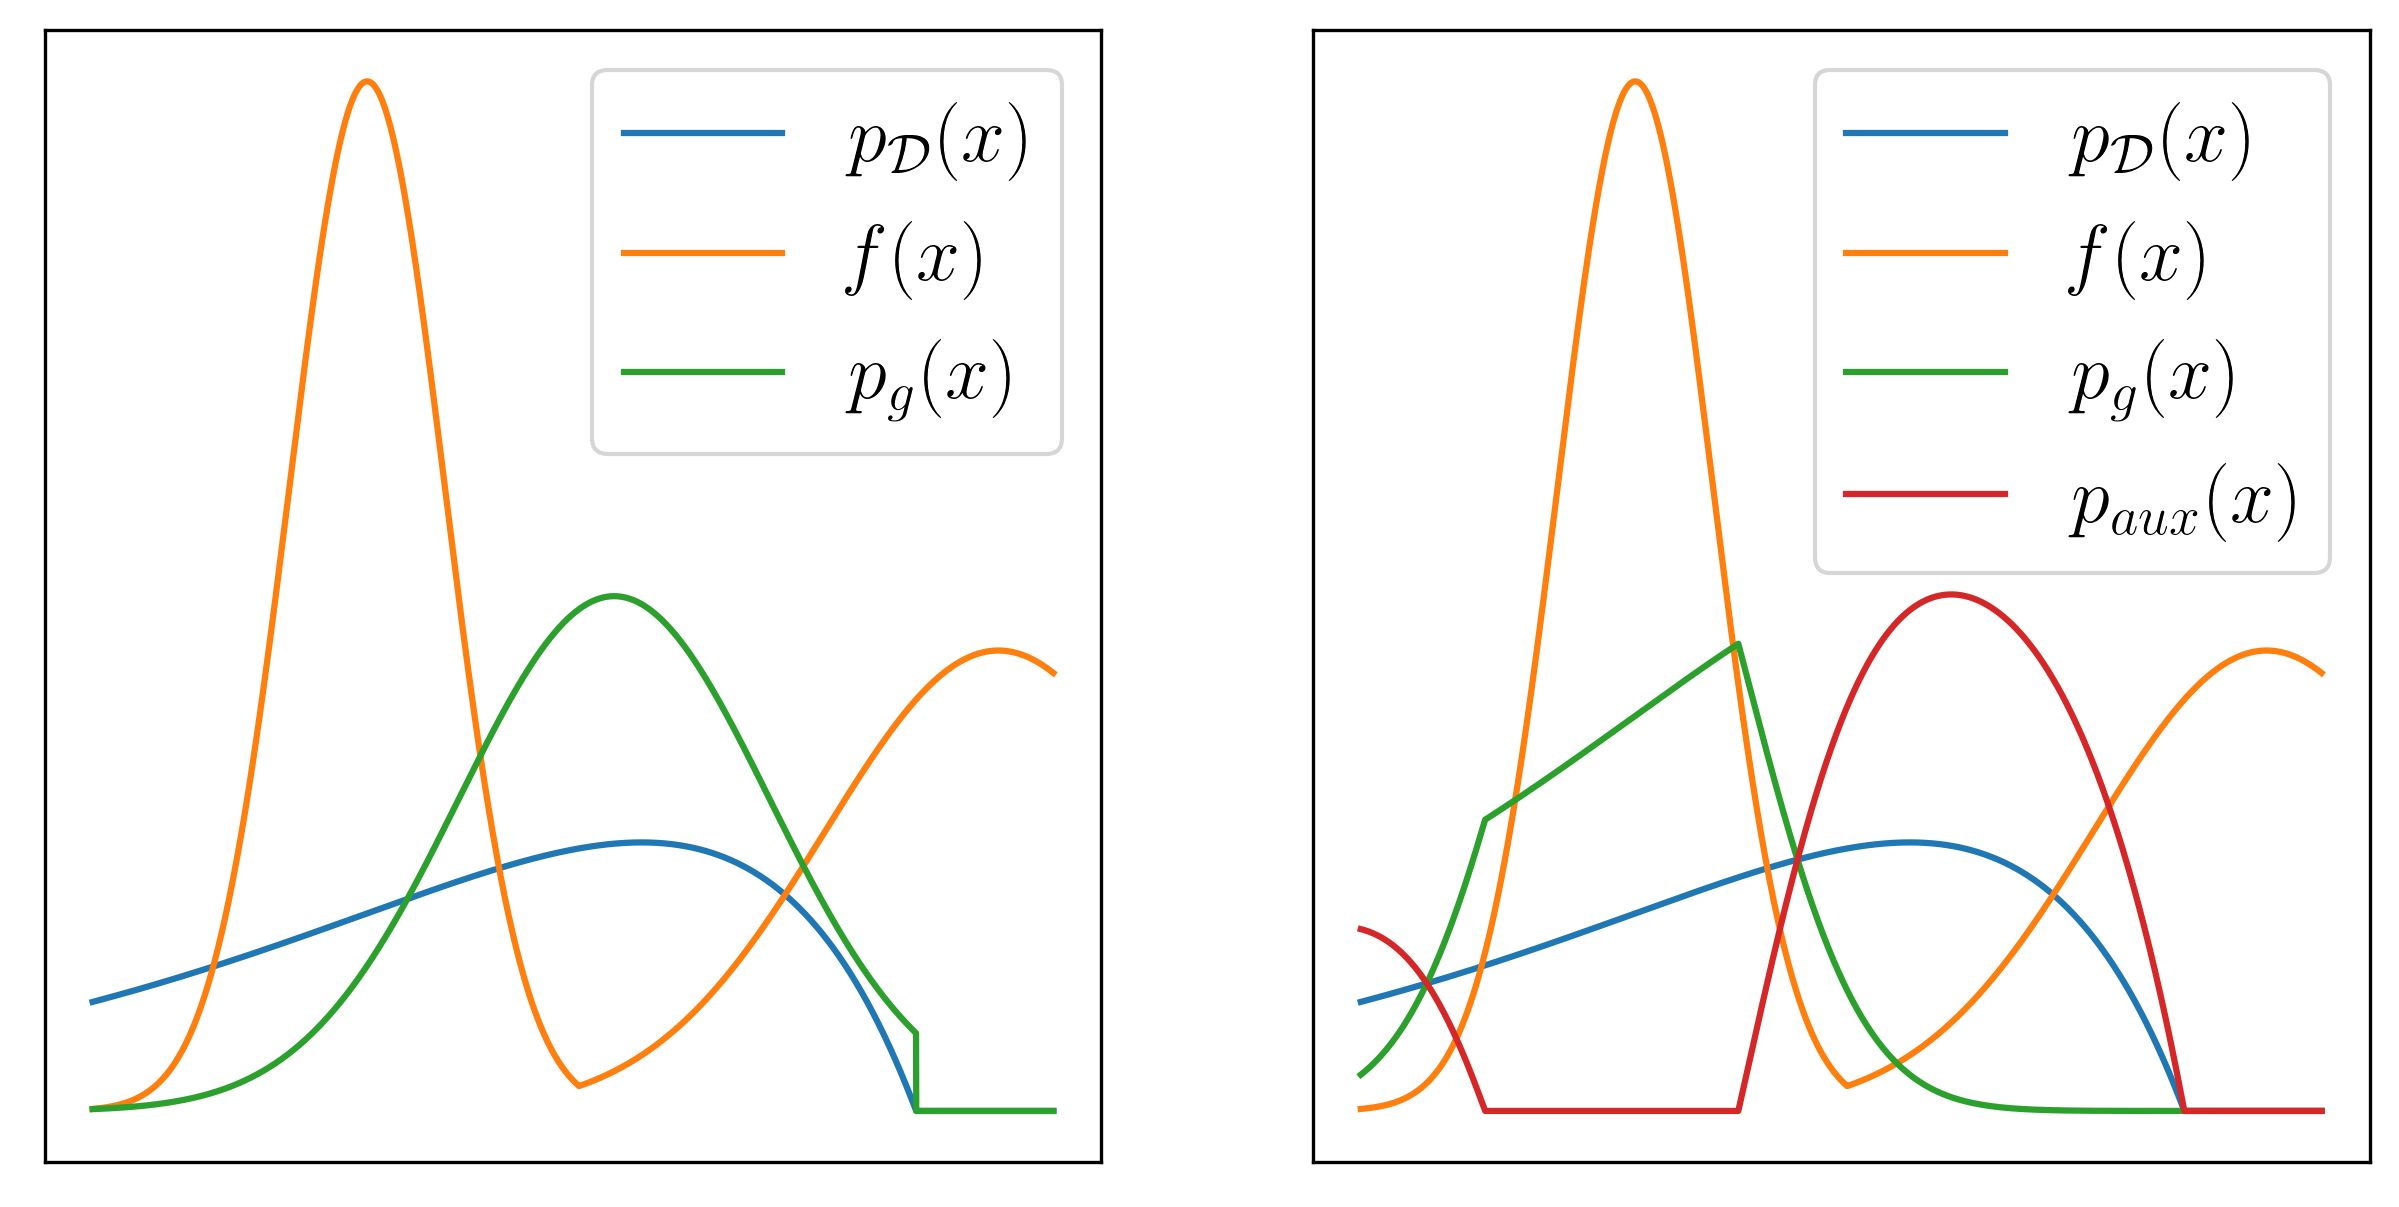
\includegraphics[width=\linewidth]{chapter_3/fig/single_and_dual.png}
  \end{center}
  \caption{Visualizations to illustrate the benefit of \textit{dual} generators over single generator when maximizing a secondary objective $f(x)$ in the GAN framework. In both figures, $p_\mathcal{D}(x)$ is the data distribution. The x-axis is a one-dimensional sample space. {\bf Left:} In this figure, since there is only a single generator, the generator $G$ is trained to jointly maximize the objective $f(x)$ and matches the data distribution $p_\mathcal{D}(x)$. The distribution $p_G$ induced by the generator is thus not very good at either maximizing the objective $f(x)$ or matching the data distribution. {\bf Right:} In this figure, we have two generators, inducing two distributions $p_G$ and $p_{aux}$. By introducing the auxiliary generator $G_{aux}$ into the GAN framework, the primary generator can better maximize the objective $f(x)$ while staying within the support of the data distribution $p_\mathcal{D}$. The mixed distribution also perfectly matches the data distribution, i.e. $ \dfrac{p_g(x) + p_{aux}(x)}{2} = p_{\mathcal{D}} (x) $. Note that in these two figures, the primary generator aims to maximize $f(x)$ (instead of minimize) to allow for more intuitive interpretation. }
  \label{fig:dual_gen_viz}
%   \vspace{-6em}
\end{wrapfigure}

% \subsection{Ensure the discriminator does not have an advantage}
In this section, we will develop an approach for performing a joint optimization of adversarial and secondary objectives of the generator in a GAN framework, which we will then apply to offline RL. This is a necessary component for performing the joint optimization in Eq.~\ref{eq:brac} without introducing a conflict of these objectives. All proofs for theorems presented in this section are in Appendix A.

Let's consider a general objective that requires training a generator $G$ to fool the discriminator $D$ while also optimizing the expected value of some other function $f$:
% \begin{align}
%     \min_{G} \max_{D}  \mathbb{E}_{ x \sim p_{\mathcal{D}}} [\log(D(x))] + \mathbb{E}_{z \sim p(z)} [\log(1-D(G(z)))]  + \mathbb{E}_{z \sim p(z)} [ f ( G(z) ) ] \label{eq:joint_nodual}
% \end{align}
\begin{align}
   \min_{G} \max_{D} \quad & \mathbb{E}_{ x \sim p_{\mathcal{D}}} [\log(D(x))] \nonumber \\
+ \hspace{0.3em} & \mathbb{E}_{z \sim p(z)} [\log(1-D(G(z)))] \nonumber \\
+ \hspace{0.3em} & \mathbb{E}_{z \sim p(z)} [ f ( G(z) ) ] \label{eq:joint_nodual}
\end{align}
where the first two terms are the same as the objective of the GAN formulation. We have also added an additional term $\mathbb{E}_{z \sim p(z)} [ f ( G(z) ) ]$, where $f$ is a mapping from the generator output to a scalar value. The third term represents a secondary objective that the generator should optimize.
\begin{restatable}{thm}{thmdisjoint}
\label{thm_disjoint}
The optimal generator of Eq.~\ref{eq:joint_nodual} induces a distribution $ p^*_g(x) = p_{\mathcal{D}} (x) \dfrac{ e^{- f(x) - \nu} }{ 2 - e^{ - f(x) - \nu } }$, where $\nu > 0$ is the Lagrange multiplier that ensures that $p^*_g(x)$ is normalized to 1.
\end{restatable}
%%SL.5.18: say where the proof for this is

We can see that by adding a secondary objective function for the generator, in general, the optimal generator does not attempt to match the data distribution $ p_{\mathcal{D}} (x) $ anymore, but instead tries to match the data distribution weighted by $ \dfrac{ e^{- f(x) - \nu } }{ 2 - e^{ - f(x) - \nu } } $. We expect that in such case, the discriminator clearly has an advantage in the two player zero-sum game and will be able to distinguish between real samples and sample generated by the generator.

To allow the generator to specialize in optimizing the secondary objective function, we propose to introduce a second auxiliary generator that matches the portion of the data distribution that is not well captured by the primary generator. Let $p_{mix} = \dfrac{ p_g + p_{aux} }{ 2 }$, consider the min-max problem:
% \begin{align}
%     \min_{G, \textcolor{red}{G_{aux}}  } \max_{D}  \mathbb{E}_{ x \sim p_{\mathcal{D}} } [\log(D(x))] + \mathbb{E}_{ \textcolor{red}{ x \sim \dfrac{ p_G + p_{aux} }{ 2 } } } [ \log(1-D(x))]  + \dfrac{1}{2} \mathbb{E}_{ x \sim p_g } [ f ( x ) ] \label{eq:joint_gan}
% \end{align}
\begin{align}
    \min_{G, G_{aux} } \max_{D}  \mathbb{E}_{ x \sim p_{\mathcal{D}} } [\log(D(x))] + \mathbb{E}_{ x \sim p_{mix} } [ \log(1-D(x))]  + \mathbb{E}_{ x \sim p_g } [ f ( x ) ], \label{eq:joint_gan}
\end{align}
%%SL.5.18: the "x \sim \dfrac{ p_G + p_{aux} }{ 2 }" looks really awkward in this Eq. -- maybe we can just define a symbol for this and use that symbol?
where we mix samples from the primary generator $G$ and the auxiliary generator $G_{aux}$ to generate samples that can fool the discriminator. The mixing is indicated by the distribution $p_{mix}$ in the second term of Eq.~\ref{eq:joint_gan}. The first and third term of Eq.~\ref{eq:joint_gan} are the same as the objective in Eq.~\ref{eq:joint_nodual}.

We next theoretically demonstrate the benefit of adding the auxiliary generator to the GAN formulation with the following Theorem.

% \begin{theorem}[Informal]
% \label{thm_joint_in_support_max}
% % Given that $f$ is appropriately bounded in its $\infty$-norm, $||f||_\infty \leq C_0 < \infty$, the primary generator $p_G$ performs in-support optimization of $f(x)$.
% % Given that $f$ is appropriately normalized, the primary generator $p_G$ performs in-support optimization of $f(x)$.
% The primary generator $p_G$ performs in-support optimization of $f(x)$.
% \end{theorem}
\begin{restatable}[Informal]{thm}{thmjointinsupportmax}
\label{thm_joint_in_support_max}
% Given that $f$ is appropriately bounded in its $\infty$-norm, $||f||_\infty \leq C_0 < \infty$, the primary generator $p_G$ performs in-support optimization of $f(x)$.
% Given that $f$ is appropriately normalized, the primary generator $p_G$ performs in-support optimization of $f(x)$.
The primary generator $p_G$ performs in-support optimization of $f(x)$.
\end{restatable}


We first note that the optimal solution of the mixed distribution from Eq.~\ref{eq:joint_gan} is the real data distribution:
\begin{align}
\dfrac{ p^*_{aux} (x) + p^*_{g} (x) }{2} = p_{\mathcal{D} } (x)
\label{eq:joint_match_real}
\end{align}
Accordingly, the optimal auxiliary generator distribution can be expressed as 
%%SL.5.18: if you find you are out of space, you can easily make some of these Eq.s inline
\begin{align}
    p^*_{aux} (x) = 2 p_{\mathcal{D}} (x) - p^*_g(x) \label{eq:paux_dist}
\end{align}
Let $x_0$ to be the element inside the support of the data distribution $p_{\mathcal{D}}$ that minimizes $f$. That is: $$ x_0 = \underset{x \in \text{Supp}( p_{\mathcal{D}} ) }{\arg\min} f(x) $$
When optimizing the secondary objective $f(x)$, the primary generator will maximize the probability mass of in-support samples that maximize $f(x)$. However, Eq.~\ref{eq:paux_dist} introduces a constraint that enforces $ 2 p_{\mathcal{D}} (x) - p^*_g(x) \geq 0$ for $p^*_{aux} (x) \geq 0$ to remain a valid distribution. This leads us to conclude that the optimal primary generator $p^*_g$ assigns the following probability to $x_0$:
% This leads us to the following definition of the in-support global maximum $x_0$ of $f(x)$:
%%SL.5.18: Perhaps we need to rephrase the above a little -- it's not clear if this is defining what "in support global maximum" means, or if it's stating a theorem saying what p*_g will learn. In fact, it's actually kind of doing both, which is really awkward -- it's simultaneously a definition for in-support max (left side) and stating a result without proof (right side). Maybe split this into a definition for in-support and a theorem statement (the right side) with proof in the appendix?
\begin{align}
    p^*_{g} (x_0) & = \begin{cases}
    2p_{\mathcal{D}} (x_0) \quad  \text{if} \quad 2p_{\mathcal{D}} (x_0) < 1 \\
    1 \quad \quad  \quad \quad \text{otherwise}
    \end{cases}
\end{align}
Interestingly, if the global maximum $x_0$ is not taking the full probability mass, the rest of the probability mass is redistributed to the next best in-support maxima, which we can define recursively:
\begin{align}
         \text{For} \,\, x_i \in \underset{x \in \text{Supp}( p_{\mathcal{D}} )  \setminus \{ x_j \}_{j=0}^{i-1} }{\arg\min} f(x), \,\,
    p^*_{g} (x_i) & = \begin{cases}
      2p_{\mathcal{D}} (x_i)\quad \quad \quad \quad \quad \text{if} \quad \sum_{j=0}^i p^*_g(x_j) < 1 \\
      1 -  \sum_{j=0}^{i-1} p^*_g(x_j) \quad \,\, \text{if} \quad \sum_{j=0}^i p^*_g(x_j) > 1 \\ 
      0 \quad \quad \quad \quad \quad \quad \quad \quad  \text{if} \quad \sum_{j=0}^{i-1} p^*_g(x_j) = 1 
    \end{cases}
    \label{eq:sol_3_cases}
\end{align}

We provide more explanation for the solution in Eq.~\ref{eq:sol_3_cases}. 
In the first case, $p^*_{g} (x_i) = 2p_{\mathcal{D}} (x_i)$ if $\sum_{j=0}^i p^*_g(x_j) < 1$. 
That is, if the optimal solution for the primary generator $p^*_{g}$ \textit{can} assign the probability $2p_{\mathcal{D}} (x_i)$ to the $i^{th}$ in support minima of $f(x)$ without the total sum of probability assigned $\sum_{j=0}^i p^*_g(x_j)$ going over $1$, then the primary generator $p^*_{g}$ will assign the probability $2p_{\mathcal{D}} (x_i)$ to $x_i$. 

In the second case, $p^*_{g} (x_i) = 1 -  \sum_{j=0}^{i-1} p^*_g(x_j)$ if $\sum_{j=0}^i p^*_g(x_j) > 1$. That is, if by assigning the probability $2p_{\mathcal{D}} (x_i)$ to the $i^{th}$ in support minima of $f(x)$, the total sum of probability assigned $\sum_{j=0}^i p^*_g(x_j)$ \textit{goes over} $1$, then the primary generator $p^*_{g}$ will assign the remaining probability $1 -  \sum_{j=0}^{i-1} p^*_g(x_j)$ to $x_i$. In the third case, the generator assigns probability $0$ to $x_i$ because all the probability has already been assigned. 
% \begin{theorem}
% The optimal solutions for the primary and secondary generators are:
% \begin{align}
%     p^*_{aux} (x) & = 2 p_{\mathcal{D}} (x) - p^*_g(x) \\
%     \text{For} \quad x_0 \in \underset{x \in Supp( p_{\mathcal{D}} ) }{argmax} f(x), \quad 
%     p^*_{g} (x_0) & = \begin{cases}
%     2p_{\mathcal{D}} (x_0) \quad  \text{if} \quad 2p_{\mathcal{D}} (x_0) < 1 \\
%     1 \quad \text{otherwise}
%     \end{cases} \\ 
%      \text{We then define $p^*_{g}$ recursively, for }  x_i \in \underset{x \in Supp( p_{\mathcal{D}} )  \setminus \{ x_j \}_{j=0}^{i-1} }{argmax} f(x): \\
%     p^*_{g} (x_i) & = \begin{cases}
%       2p_{\mathcal{D}} (x_i) \quad \text{if} \quad \sum_{j=0}^i p^*_g(x_j) < 1 \\
%       1 -  \sum_{j=0}^{i-1} p^*_g(x_j) \quad \text{if} \quad \sum_{j=0}^i p^*_g(x_j) > 1 \\ 
%       0 \quad \quad \text{if} \quad \sum_{j=0}^{i-1} p^*_g(x_j) = 1 
%     \end{cases}       
% \end{align}
% \end{theorem}
%     % p^*_{g} (x) & = \dfrac{1}{Z_{G}} \left[ 2 p_{\mathcal{D} } (x) \dfrac{ e^{2f(x)} }{ 2 - e^{ 2f(x) } } - p^*_{aux} (x) \right] 

% \textcolor{red}{Does anyone have a nicer way to write the expression above}.

% \textcolor{red}{TODO: show that the dual generator optimal solution is indeed preferable to single generator, maybe in terms of well the primary generator can maximize E[f(x)]}. We probably need to introduce a mixing weight $\alpha$ between the two generators show this.

% TODO: provide some intuition about why the solution for $p^*_g$ looks like that, this is because $p^*_{aux} (x) = 2 p_{\mathcal{D}} (x) - p^*_g(x) \geq 0$, so $p^*_g(x)$ can be at most $2p_{\mathcal{D}} (x)$. And $p_{\mathcal{D}} (x) = 0 \implies p^*_{aux} (x) = p^*_g(x) = 0 $. As such, let $x_0$ be the global maxima of $f(x)$ that lies within the support of $p_{\mathcal{D}}$, we set the probability of the global maxima to be $2p_{\mathcal{D}}(x_0)$. If this value is less than 1, that means we still have probability mass left to redistribute. We then consider the next global maxima $x_1$ of $f(x)$ that lies within the support of $p_{\mathcal{D}}$, excluding $x_0$, and set the probability of the $p^*_{g} (x_1)$ to be $2p_{\mathcal{D}}(x_0)$. So on until we run out of probability mass to redistribute.

% \begin{corollary}
% $ \dfrac{ p^*_{aux} (x) + p^*_{g} (x) }{2} = p_{\mathcal{D} } (x) $
% \end{corollary} 


To summarize the benefit of dual generator, we note that by introducing an auxiliary generator and mixing it with the primary generator, not only does the optimal solution for the mixed distribution match the real data distribution, but also the primary generator can better optimize the secondary objective $f$ on the part of the domain of $f$ that is within the support of the data distribution $p_\mathcal{D}$. To better illustrate the benefit, we provide a visual explanation of the benefit in Figure~\ref{fig:dual_gen_viz}.
% in-distribution support.

% \begin{theorem}
% By allowing in-support optimization of $f(x)$, using the auxiliary generator enables the primary generator to better optimize the secondary objective $f(x)$ compared to not using the auxiliary generator and only using a single generator.
% \end{theorem}
% %%SL.5.18: we probably need a more formal statement here than just "better"
% That is, let $p_{\mathlarger{g}}^*$ be the distribution induced by the optimal generator obtained from Eq.~\ref{eq:joint_gan} where we use the auxiliary generator. Also let $p_{\mathlarger{s}}^*$ be the distribution induced by the optimal generator obtained from Eq.~\ref{eq:joint_nodual}, where we do not use the auxiliary generator. We are then interested in showing that:
% \begin{align*}
%     \mathbb{E}_{ x \sim p_{\mathlarger{g}}^* } [ f ( x ) ] \geq \mathbb{E}_{ x \sim p_{\mathlarger{s}}^* } [ f ( x ) ]
% \end{align*}
%%SL.5.18: I think the above should all be part of the theorem? that woudl make it more precise, then say where the proof is...

% We next illustrate the benefit of introducing the auxiliary generator on a toy 2D task.

% In this subsection, we show that by using a single generator, the discriminator has an advantage because the generator is not even trying to match the data distribution.

% That is, when there is a secondary objective function and we only use a single generator, then the optimal solution for the generator does not try to match the data distribution p\_data, which is what a GAN Generator should do.

% We then show that by introducing the second auxiliary generator, the mixed distribution of the first and the second generator is trying to match the data distribution, and hence the discriminator does not have an advantage anymore.

% More info: pls see file 'discriminator does not have advantage.pdf' for derivation and file 'GAN dual discriminator toy example.pdf' for the toy example

% \subsection{Support Constraint}

% In this subsection, we show a second benefit of having the second auxiliary generator. "I can show that for 2 different actions, if they have the same probability under the behavior policy, and one has higher Q value, then by having two generators, the policy can assign more mass to the higher action, as compared to when there is only one generator!"

\subsection{Update rules for offline reinforcement learning}
\label{sec:update_rule}

We will now incorporate the dual-generator method to train policies for offline RL, based on optimizing the joint objective from Eq.~\ref{eq:joint_gan}. The updates for the actor and the critic are generally similar to Eq.~\ref{eq:brac_update}. However, simply combining Eq.~\ref{eq:joint_gan} and Eq.~\ref{eq:brac_update} can still allow the policy to exploit errors in the value function during the policy improvement step. We therefore augment the policy improvement step with an adaptive weight on the Q-value.
%%SL.5.18: Maybe it would be better to have a separate subsection before this that first motivates and then explains the weighting, and then have this section just be a "putting it together" kind of algorithm summary? Or we can keep it as-is, but then it would be good to motivate the weighting somewhere before this, otherwise it's pretty surprising that we're not just plugging the Sec 4.1 thing in here but doing something more complex. Perhaps that could be done simply by taking some of the motivation that is already here and putting it earlier? Or just explicitly say that we could simply plug the GAN from 4.1 into actor-critic Eq ??, but this would have a problem, so we also do this weight (which would be most similar to the current phrasing, just a bit more explicit)
More concretely, as the policy improvement step samples actions from the current policy iterate $\policy^k$ to optimize the policy objective, there is a non-zero probability that the sampled actions will exploit spurious maxima in the value function and have their probability of being sampled again in the future increased. If the same actions are sampled during the policy evaluation step, the errors in the value functions from the next states are backed up into the preceding states, leading to divergent value functions, as we observe in our experiments. To alleviate this issue, we use the probability assigned to the sampled actions by the discriminator to weight the value function estimates in the policy objective, leading to the following updates:
\begin{align}
    Q^{k+1} \leftarrow& \argmin_{Q} \E_{s, a, s' \sim \mathcal{D}}\left[ \left((R(s, a) +  \gamma \E_{a' \sim {\policy}^k(a'|s')}[Q^{k}(s', a')]) - Q_{target}(s, a)\right)^2 \right] \label{eq:dasco_q}\\ 
    \policy^{k+1} \leftarrow& \argmax_{\policy} \E_{s, a_{\mathcal{D}} \sim \mathcal{D}, a \sim \policy^k(a|s)}\left[ \dfrac{ D^k(s,a) }{ D^k( s,a_{\mathcal{D}}(s)) }Q^{k+1}(s, a) + \log D^k(s,a) \right],
    \label{eq:dasco_pi}
\end{align}
where $ a_{\mathcal{D}}(s) $ is the action from the offline dataset. 
%The state $\bs$ is sampled from the offline dataset. The action $\ba$ is sampled from the $k^{th}$ policy iterate $ \pi^k_\phi $. 
The term $ D^k(s,a) $ down-weights the contribution of the gradient of the value function to the policy update if the discriminator deems the sampled action too unlikely. We further calibrate the probability $ D^k(s,a) $ by dividing it with the probability $ D^k(s,a_{\mathcal{D}}(s)) $ that the discriminator assigns to the dataset action $a_{\mathcal{D}}(s) $. It should be noted that during optimization the gradients are not propagated into these weights.%\autoref{eq:update_dynamic_weight} illustrate the update rule using a single state from the dataset for clarity. In practice, we average the gradient over multiple states and also incorporate a learning rate.

Next, we define the update rules for the auxiliary generator and the discriminator. We mix the samples from the $k^{th}$ iterate of the policy $\pi^k$ and the distribution $p_{aux}$ induced by the $k^{th}$ iterate of the auxiliary generator $G^k_{aux}$, that is, let $p_{mix} = \dfrac{ \pi^k + p_{aux} }{ 2 }$. At every iteration $k$, we update the $k^{th}$ iterate of the auxiliary generator $ G^{k}_{aux} $ and discriminator $D^k$ using the objectives:
\begin{align}
    G^{k+1}_{aux} \leftarrow& \argmin_{ G_{aux} } \mathbb{E}_{ x \sim p_{mix} } [ \log(1-D^k(s,a))] \label{eq:dasco_gaux}\\ 
    D^{k+1}  \leftarrow& \argmax_{D}  \mathbb{E}_{ x \sim p_{\mathcal{D}} } [\log(D^k(s,a))] + \mathbb{E}_{ x \sim p_{mix} } [ \log(1-D^k(s,a))]\label{eq:dasco_d}
    %%SL.5.18: same comment about the akwardness of the giant mixture Eq. in the subscript
\end{align}
%%SL.5.18: perhaps pseudocode summarizing the whole algorithm would be useful? maybe together with a short paragraph after this that just rounds out all the pieces and summarize the whole thing
\subsection{Algorithm summary}
\label{sec:algo_summary}

Algorithm ~\ref{algo:dasco} provides a step-by-step description of our algorithm. At every training step, we sample a batch of transitions from the offline dataset and proceed to update the parameters of the value function, the policy, the auxiliary generator and the discriminator in that order.

\begin{algorithm}[H]
\begin{algorithmic}[1]
\State{Initialize Q-function $Q_\theta$, policy $\pi_\phi$, auxiliary generator $G_{aux, \psi}$, discriminator $D_\omega$}
\For{training step $k$ in \{1,\dots,N\}}
\State{$(s, a, r, s') \gets \mathcal{D}$: Sample a batch of transitions from the dataset}
\State{$\theta^{k+1} \gets$ Update Q-function $Q_\theta$ using the Bellman update in Eq.~\ref{eq:dasco_q}}
\State{$\phi^{k+1} \gets$ Update policy $\pi_\phi$ using the augmented objective in Eq.~\ref{eq:dasco_pi}}
\State{$\psi^{k+1} \gets$ Update auxiliary generator $G_{aux, \psi}$ using the objective in Eq.~\ref{eq:dasco_gaux}}
\State{$\omega^{k+1} \gets$ Update discriminator $D_\omega$ using mixed samples from $\pi_\phi$ and $G_{aux, \psi}$ as in Eq.~\ref{eq:dasco_d}}
\EndFor
\caption{\name{} algorithm summary}
\label{algo:dasco}
\end{algorithmic}
\end{algorithm}

\section{Experiments}
\label{sec:dasco_exp}

% \renewcommand{\arraystretch}{1.2}

% Our experiments aim at answering the following questions: 1. When learning from offline datasets that require combining actions from sub-optimal trajectories, does \name{} outperform existing methods that are based on distribution constraints? 2. On standard benchmarks such as D4RL~\cite{d4rl}, how does \name{} compare against recent methods? 3. Are both the dual generator and the probability ratio weight important for the performance of \name{}?

Our experiments aim at answering the following questions: 
\begin{enumerate}
    \item When learning from offline datasets that require combining actions from sub-optimal trajectories, does \name{} outperform existing methods that are based on distribution constraints? 
    \item On standard benchmarks such as D4RL~\cite{d4rl}, how does \name{} compare against recent methods? 
    \item Are both the dual generator and the probability ratio weight important for the performance of \name{}?
\end{enumerate}

\subsection{Comparisons on standard benchmarks and new datasets}
%%SL.5.18: Maybe we can start with a short discussion (a sentence or two) for why we need to add the new tasks? I also wonder if the subsection title might be perceived as a little misleading, since it says comparisons on d4rl tasks, but then the discussion talks about creating new tasks that are not the d4rl tasks...

For our first set of experiments, we introduce four new datasets to simulate the challenges one might encounter when using offline RL algorithms on real world data. These datasets introduce additional learning challenges and require the algorithm to combine actions in different trajectories to obtain good performance. We use the existing AntMaze environments from the D4RL suite~\cite{d4rl}: antmaze-medium and antmaze-large. In these two environments, the algorithm controls an 8-DoF ``Ant" quadruped robot to navigate a 2D maze to reach desired goal locations. 
The D4RL benchmark generates the offline datasets for these two environments using two policies: 1. a low-level goal reaching policy that outputs torque commands to move the Ant to a nearby goal location and 2. a high-level waypoint generator to provide sub-goals that guide the low-level goal-reaching policy to the desired location.
We use the same two policies to generate two new classes of datasets. 

For the \texttt{noisy}
dataset, we add Gaussian noise to the action computed by the low-level goal-reaching policy. The noise variance depends on the 2D location of the Ant in the maze -- larger in some 2D regions than others. We intend this dataset to be representative of situations where the data generation policies are more deterministic in some states than others~\cite{kumar2022prefer} -- a robot picking up an object has many good options to approach the object, but when the robot grasps the object, its behavior should be more deterministic to ensure successful grasp without damaging or dropping the object \cite{10.5555/561828}.
% a robot navigating a room have many degree of freedom of movements, but once it crosses through a door, there is a much smaller set of actions that allow it to successfully navigate through the constrained free space. 
%%SL.5.18: I'm having some difficulty following the intuition in this last sentence.

For a \texttt{biased} dataset, in addition to adding Gaussian noise to the actions as it is done in the \texttt{noisy} dataset, we also add  bias to the actions computed by the low-level policy. The values of the bias also depend on the current 2D location of the Ant in the maze. This setting is meant to simulate learning from relabelled data, where the dataset was generated when the data generation policies were performing a different task than the tasks we are using the dataset to learn to perform. Relabelling offline data is a popular method for improving the performance of offline RL algorithms \cite{MBRL, Snell2022}, especially when we have much more data for some tasks than others \cite{mtopt}.
In the AntMaze environment, offline RL algorithms must combine data from sub-optimal trajectories to learn behaviors with high returns. In addition, \texttt{noisy} and \texttt{biased} datasets present a more challenging learning scenarios due to the added noise and systematic bias which vary non-uniformly based on the 2D location of the Ant.

\autoref{tab:hetero_antmaze} illustrates the performance comparison of our method and representative methods that enforce distribution constraints, either through optimizing a conservative lower bound of the value estimates (CQL) or only optimizing the policy on actions in the dataset using Advantage Weighted Regression \cite{peng2019awr} (IQL). Our method outperforms both CQL and IQL. In these tasks, to ensure a fair comparison between  different methods, we perform oracle offline policy selection to obtain the performance estimates for CQL, IQL, and our method. We also compare the performance on standard AntMaze tasks when learning from the datasets in the D4RL benchmark without modifications in \autoref{tab:d4rl_antmaze}. In these tasks, our method outperforms IQL by a large margin on two diverse datasets.
\begin{table}[!htp]\centering
\caption{Performance comparison to distribution-constrained baselines when learning from the \texttt{noisy} and \texttt{biased} datasets. Our method outperforms the baselines by a large margin.}\label{tab:hetero_antmaze}
%%SL.5.18: Here and elsewhere, I would suggest trying to make the caption a bit more informative. A good idea for the caption is to have one sentence describing what the figure shows, and then another sentence or two explaining what the reader should look for in the figure. For space constraints, you can probably find a way to put Table 1 and Table 2 side-by-side; it may also be good to bold the best result in the tables (though if they are close, consider if we can somehow get error bars and only bold differences that are statistically significant)
\small
\begin{tabular}{l||rr|r}
Dataset & CQL & IQL & \name{} (Ours) \\ \hline

% name in code is antmaze-large-recollect-actually-v2 &  & 41.0 (7.9) & \textbf{} \\
antmaze-large-bias & 50.0 & 41.0 & \textbf{ 63.9 } \\

% name in code is antmaze-large-recollect-v2  &  & 39.0 (6.4) & \textbf{} \\
antmaze-large-noisy  & 41.7 & 39.0 & \textbf{ 54.3 } \\

% antmaze-medium-recollect-actually-v2  & & 48.0 (5.9) & \textbf{} \\
antmaze-medium-bias  & 72.7 & 48.0 & \textbf{ 90.2 } \\

% antmaze-medium-recollect-v2  & & 44.3 (1.7) & \textbf{} \\ \hline
antmaze-medium-noisy  & 55.0 & 44.3 & \textbf{ 86.3 } \\ \hline

\texttt{noisy} and \texttt{biased} antmaze-v2 total & 219.4 & 172.3 &  \textbf{294.7} \\ \hline
\end{tabular}
\end{table}
% IQL and Ours taken from https://docs.google.com/spreadsheets/d/1rAZkYLL2SkzskYdbF-oVQ2GjQ1RMifJb0Sr_DLITi6g/edit#gid=920938660
% CQL from https://wandb.ai/aviralkumar/Antmaze-runs-with-full-orthogonal-init-randomized-DR3-runs--UpdateD4RL-AndDR3-antmaze?workspace=user-aviralkumar
\begin{table}[!htp]\centering
\caption{Performance comparison to distribution-constrained baselines on AntMaze tasks in D4RL. Our algorithm outperforms the baselines when learning from two diverse datasets.}\label{tab:d4rl_antmaze}
\small
\begin{tabular}{l||rr|r}
Dataset  &CQL & IQL & \name{} (Ours) \\\hline
antmaze-umaze & 95.0 & 93.0 & 98.2  \\
antmaze-umaze-diverse  & 61.0 & 64.0 & \textbf{97.1} \\
antmaze-medium-play & 73.0 & 82.0 & 87.8 \\
antmaze-medium-diverse & 73.2 & 81.0 & 84.6 \\
antmaze-large-play & 44.0 & 53.0 & 56.0 \\
antmaze-large-diverse & 46.0 & 53.0 & \textbf{74.1} \\ \hline
antmaze total & 392.2 & 426.0 & 497.8 \\ 
\hline 
\end{tabular}
\end{table}
\begin{table}[!htp]\centering
\caption{Performance comparison with recent offline RL algorithms on the Gym locomotion tasks}\label{tab:d4rl_locomotion}
\scriptsize
\setlength{\tabcolsep}{0.7em}
\begin{tabular}{l||rrrrrrrr|r}
Dataset &BC &10\%BC &DT &AWAC &Onestep RL &TD3+BC &CQL & IQL & \name{} (Ours) \\\hline
halfcheetah-medium-replay & 36.6 &40.6 &36.6 &40.5 &38.1 & 44.6 & 45.5 & 44.2 & 44.7  \\
hopper-medium-replay & 18.1 &75.9 &82.7 &37.2 & 97.5 &60.9 & 95.0 & 94.7 & 101.7  \\
walker2d-medium-replay & 26.0 &62.5 &66.6 &27.0 &49.5 & 81.8 &77.2 & 73.9 & 74.5 \\
halfcheetah-medium-expert & 55.2 & 92.9 &86.8 &42.8 & 93.4 & 90.7 & 91.6 & 86.7 & 94.3  \\
hopper-medium-expert & 52.5 & 110.9 & 107.6 &55.8 &103.3 &98.0 & 105.4 &91.5 & 111.4 \\
walker2d-medium-expert & 107.5 & 109.0 & 108.1 & 74.5 & 113.0 & 110.1 & 108.8 & 109.6 & 109.3  \\ \hline
locomotion total & 295.9 & 491.8 & 488.4 & 277.8 & 494.8 & 486.1 & 523.5 & 500.6 & 535.9 \\
\hline
\end{tabular}
\end{table}


By comparing the results in \autoref{tab:hetero_antmaze} (learning from \texttt{noisy} and \texttt{biased} datasets) and \autoref{tab:d4rl_antmaze} (learning from existing offline datasets in D4RL), we also note that our proposed algorithm outperforms distribution-constraint offline RL algorithms (CQL, IQL) more consistently when tested on the \texttt{noisy} and \texttt{biased} datasets. For the results in these two tables, the definition of the antmaze-medium and antmaze-large environments are the same. The only axis of variation in the learning setup is the noise and systematic bias added to the actions of the dataset generation policies. We therefore conclude that our algorithm is more robust to the noise and systematic bias added to the actions than distribution-constrained offline RL algorithms.

% Our methods outperform baselines by a larger margin when the algorithms learn from the 
% Since the environment definition is the same across the antmaze-large and antmaze-medium tasks in \autoref{tab:hetero_antmaze} and \autoref{tab:d4rl_antmaze},
%%SL.5.18: I don't quite understand the significance of "environment definition is the same" here...

Next, we evaluate our approach on Gym locomotion tasks from the standard D4RL suite. The performance results on these tasks are illustrated in \autoref{tab:d4rl_locomotion}. Our method is competitive with BC, one-step offline RL methods \cite{brandfonbrener2021offline}, and multi-step distribution-constraint RL  methods \cite{kostrikov2021offline, kumar2020conservative}. This is not surprising because in these tasks, the offline dataset contains a large number of trajectories with high returns.
%%SL.5.18: you mean 10% BC? regular BC performs horribly...
%We present the result on the Adroit dexterous manipulation tasks in the Appendix.

In terms of total amount of compute and type of resources used, we use an internal cluster that allows for access up to 64 preemptive Nvidia RTX 2080 Ti GPUs. For each experiment of learning from an offline dataset, we use half a GPU and 3 CPU cores. Each experiment generally takes half a day to finish. We implemented our algorithms in Pytorch~\cite{paszke2019pytorch} and obtained results for baselines from the publicly available implementations released by the original authors. 
% Regarding hyper-parameter tuning, we tune the hyper-parameters for the GAN, including instance noise 

% On the Adroit dexterous manipulation tasks, previous offline RL methods have only been shown to be competitive with BC. This is because the offline datasets contain mostly demonstrations. Our method is no different and we therefore include the results on the Adroit tasks in the Appendix.
%%SL.5.18: I think we can just keep these last two sentences short and say that we present the others in the appendix, it would be a good idea not to distract the reader with extraneous information, and instead add a few concluding sentences after this about what the main takeaways from the experiments should be

% 36.6 + 18.1 + 26.0 + 55.2 + 52.5 + 107.5 = 295.9
% 40.6 + 75.9 + 62.5 + 92.9 + 110.9 + 109.0 = 491.8
% 36.6 + 82.7 + 66.6 + 86.8 + 107.6 + 108.1 = 488.4
% 40.5 + 37.2 + 27.0 + 42.8 + 55.8 + 74.5 = 277.8
% 38.1 + 97.5 + 49.5 + 93.4 + 103.3 + 113.0 = 494.8
% 44.6 + 60.9 + 81.8 + 90.7 + 98.0 + 110.1 = 486.1
% 45.5 + 95.0 + 77.2 + 91.6 + 105.4 + 108.8 = 523.5
% 44.2 + 94.7 + 73.9 + 86.7 + 91.5 + 109.6 = 500.6
% 44.7 + 101.7 + 74.5 + 94.3 + 111.4 + 109.3 = 535.9



% \subsection{Fine-tuning experiments}

\subsection{Ablations}

%%SL.5.18: if you end up short on space, this paragraph is a great candidate for shortening
We conduct three different sets of experiments to gain more insights into our algorithm. The first experiment measures the importance of having an auxiliary generator. We recall that there are two benefits to having the auxiliary generator. Firstly, without the auxiliary generator, the generator does not in general match the data distribution (\autoref{thm_disjoint}). As such, the discriminator has an unfair advantage in learning how to distinguish between real and generated examples. Secondly, the auxiliary generator plays the role of a support player and learns to output actions that are assigned non-zero probability by the data distribution, but have low Q values. The support player allows the policy to concentrate on in-support maximization of the Q-function (\autoref{thm_joint_in_support_max}). \autoref{tab:abs_aux_gen} demonstrates that having an auxiliary generator clearly leads to a performance improvement across different task families, from Gym locomotion tasks to AntMaze tasks and even dexterous manipulation tasks.

The second experiment compares the performance of the policy and the auxiliary generator on a subset of the Gym locomotion and AntMaze tasks (\autoref{tab:policy_vs_aux}). The difference in the performance of the policy and auxiliary generator illustrates their specialization of responsibility: the policy learns to output actions that lead to good performance, while the auxiliary generator learns to model the ``remainder" of the data distribution. If this ``remainder" also contains good action, then the auxiliary generator will have non-trivial performance. Otherwise, the auxiliary generator will have poor performance. 

In the Gym locomotion tasks, the auxiliary generator has non-trivial performance, but it is still worse than the policy. This demonstrates that: 1. By optimizing the policy to maximize the long-term return and the discriminator function, the policy can outperform the auxiliary generator, which only maximizes the discriminator function, 2. The dataset contains a large fraction of medium performance level actions contained in continuous trajectories, which the auxiliary generator has learnt to output. In contrast, in the \texttt{bias} and \texttt{noisy} AntMaze tasks, the auxiliary generator fails to obtain non-zero performance while the policy has strong performance. This reflects the necessity of carefully picking a subset of the in-support actions to obtain good performance.
%%SL.5.18: My sense is that these experiments are kind of in the opposite order. The important question is whether the auxiliary generator helps, so it makes sense to put that first. Then you could discuss *why* it's interesting to try to use the auxiliary generator as a policy, and then show those results. In general, remember also to motivate why each experiment is being conducted and then discuss the implications/takeaways from that experiment.


% /quan-fast-vol/google/ongoing_exp/April_26/gaussian
% /home/tele_mani_u20/code_proj/google/gan_for_state_matching/ongoing_exp/april5/brute_force_search_no_date_in_logdir
\begin{table}[!htp]\centering
\caption{Ablation for training without and with auxiliary generator. The dual generator technique, which trains the auxiliary generator in addition to the policy, is crucial to obtain good performance.}\label{tab:abs_aux_gen}
\small
\begin{tabular}{l||rr}
Dataset & Without & With \\ \hline

halfcheetah-medium-expert & 77.7 &  94.3\\
hopper-medium-expert & 99 & 111.4 \\ 

% name in code is antmaze-large-recollect-actually-v2 &  & 41.0 (7.9) & \textbf{} \\
antmaze-large-bias & 54.0 & 63.9 \\

% name in code is antmaze-large-recollect-v2  &  & 39.0 (6.4) & \textbf{} \\
antmaze-large-noisy & 39.0 & 54.3 \\


relocate-human-longhorizon & 10.1 & 40.7 \\ 

\hline
\end{tabular}
\end{table}


% /quan-fast-vol/google/ongoing_exp/May_08/antmaze_new_dist_after_data_collect_bug_fix/logs/aggregate_perf/2022-05-17 21:51:36.371325/antmaze_newrelabel/debug.log
\begin{table}[!htp]\centering
\caption{Policy vs Auxiliary Generator. The auxiliary generator has reasonable performance on the easier locomotion tasks and is significantly worse than the policy on the harder AntMaze tasks.}\label{tab:policy_vs_aux}
\small
\begin{tabular}{l||rr}
Dataset & Auxiliary Generator & Policy \\ \hline

halfcheetah-medium-expert & 44.167 & 94.3 \\
hopper-medium-expert & 75.357 & 111.4 \\
% walker2d-medium-expert-v2 & 96.562 & 109.3 \\

% name in code is antmaze-large-recollect-actually-v2 &  & 41.0 (7.9) & \textbf{} \\
antmaze-large-bias & 0.0 & 63.9 \\

% name in code is antmaze-large-recollect-v2  &  & 39.0 (6.4) & \textbf{} \\
antmaze-large-noisy  & 0.0  & 54.3 \\

% % antmaze-medium-recollect-actually-v2  & & 48.0 (5.9) & \textbf{} \\
% antmaze-medium-bias-v2  & 0.15 &  & \textbf{} \\

% % antmaze-medium-recollect-v2  & & 44.3 (1.7) & \textbf{} \\ \hlineov
% antmaze-medium-noisy-v2  & 0.15 &  & \textbf{} \\ \hline
\end{tabular}
\end{table}


The third set of experiments illustrates the importance of weighing the value function in the policy objective by the probability computed by the discriminator, as described in Eq.~\ref{eq:dasco_pi}. Doing so provides a second layer of protection against exploitation of  errors in the value function by the policy. \autoref{tab:abl_dynamic_weighting} illustrates that this is very important for the AntMaze tasks, which require combining optimal and sub-optimal trajectories to obtain good performance. Perhaps this is because learning from such trajectories necessitates many rounds of offline policy evaluation and improvement steps, with each round creating an opportunity for the policy to exploit the errors in the value estimates. 
On the other hand, the dynamic weight is less important in the Gym locomotion tasks, presumably because a significant fraction of the corresponding offline datasets has high returns and therefore incorporating sub-optimal data is less criticial to obtain high performance.

% /quan-fast-vol/google/ongoing_exp/May_08/antmaze_new_dist_after_data_collect_bug_fix/logs/aggregate_perf/2022-05-17 21:51:36.371325/antmaze_newrelabel/debug.log
\begin{table}[!htp]\centering
\caption{Ablation for dynamic weighting of value function estimates in the policy objective. When learning from datasets that require combining actions across trajectories, such as the AntMaze tasks, using the dynamic weighting is vital to obtaining good performance.}\label{tab:abl_dynamic_weighting}
\small
\begin{tabular}{l||rr}
Dataset & Without & With \\ \hline

halfcheetah-medium-expert & 89.7  & 94.3  \\
hopper-medium-expert & 110.8  & 111.4 \\
% walker2d-medium-expert-v2 & 111.6  &  \\

% antmaze-medium-play-v2 & 5.0 & \\
% antmaze-medium-diverse-v2 & 5.0 & \\
antmaze-large-play & 0.0 & 56.0 \\ 
antmaze-large-diverse & 0.0 & 74.1 \\ 

\hline
\end{tabular}
\end{table}



\section{Proofs for theorems in Section~\ref{sec:dual_gen}}

\subsection{Proof for Theorem~\ref{thm_disjoint} }

In the following proof, we use $p_{\text{data}}$ to refer to the real data distribution, instead of $p_\mathcal{D}$ as in Section~\ref{sec:dual_gen}, to avoid confusion with the discriminator distribution.

We recall Theorem~\ref{thm_disjoint}:

\thmdisjoint*

The optimization problem in Eq.~\ref{eq:joint_nodual} is:
\begin{align*}
    \min_{G} \max_{D}  V(G, D) = \mathbb{E}_{ x \sim p_{\text{data}}} [\log(D(x))] + \mathbb{E}_{z \sim p(z)} [\log(1-D(G(z)))]  + \mathbb{E}_{z \sim p(z)} [ f ( G(z) ) ]
\end{align*}

The proof proceeds as follows: We first simplify the objective function into two terms. The first term is the Jensen–Shannon divergence between the data distribution and the distribution induced by the generator~\cite{gan}. The second term is the expected value of the secondary objective function $f$. We then show that the problem is convex, where strong duality holds. We then use the KKT conditions to find the functional form of the optimal solution, which gives us Theorem~\ref{thm_disjoint}.

We only prove the statement for discrete sample space, and we let $n$ be the size of the sample space -- the random variable $x$ can take on $n$ different values.

\textit{Proof}. Since the third term in the objective function is not a function of the discriminator $D$, for $G$ fixed, the optimal discriminator of Eq.~\ref{eq:joint_nodual} is $D^*_G(x) = \dfrac{ p_{\text{data}} (x) }{ p_{ \text{data} } (x) + p_{g }(x) }$ where $p_g$ is the distribution induced by the generator $G$.
 (similar to Prop 1 in \cite{gan} ).

Similarly to how \cite{gan} shows that the GAN objective in Eq.~\ref{eq:vanilla_gan} minimizes the JS divergence between the data distribution and the distribution induced by the generator, we can now rewrite the objective in Eq.~\ref{eq:joint_nodual} as:
\begin{align}
     & V(G, D^*_G)\\
     & = \mathbb{E}_{ x \sim p_{\text{data}}} [\log(D^*_G(x))] + \mathbb{E}_{z \sim p(z)} [\log(1-D^*_G(G(z)))]  + \mathbb{E}_{z \sim p(z)} [ f ( G(z) ) ] \\
    %  & = \mathbb{E}_{ x \sim p_{\text{data}}} [\log(D^*_G(x))] + \mathbb{E}_{x \sim p_g} [\log(1-D^*_G(x))]  + \mathbb{E}_{z \sim p(z)} [ f ( G(z) ) ] \\
    %  & = \mathbb{E}_{ x \sim p_{\text{data}}} [\log( \dfrac{ p_{\text{data} }(x) }{ p_{\text{data} } (x) + p_{ g } (x) } )] + \mathbb{E}_{x \sim p_g} [\log(1 - \dfrac{ p_{\text{data} } (x) }{ p_{ \text{data} } (x) + p_{g } (x) } )]  + \mathbb{E}_{x \sim p_g} [ f ( x ) ] \\
    %  & = \mathbb{E}_{ x \sim p_{\text{data}}} [\log( \dfrac{ p_{\text{data} }(x) }{ p_{\text{data} } (x) + p_{ g } (x) } )] + \mathbb{E}_{x \sim p_g} [\log( \dfrac{ p_g (x) }{ p_{ \text{data} } (x) + p_{ g } (x) } )] + \mathbb{E}_{x \sim p_g} [ f ( x ) ] \\
    %  & = \mathbb{E}_{ x \sim p_{\text{data}}} [\log( \dfrac{ p_{\text{data} }(x) }{ ( p_{\text{data} } (x) + p_{ g } (x) ) / 2 } ) - \log 2] + \mathbb{E}_{x \sim p_g} [\log( \dfrac{ p_g (x) }{ ( p_{ \text{data} } (x) + p_{ g } (x) ) / 2 } ) - \log 2]  + \mathbb{E}_{x \sim p_g} [ f ( x ) ] \\ 
    %  & = KL \left( p_{\text{data}} || \dfrac{ p_{\text{data} } (x) + p_{ g } (x) }{ 2 } \right) + KL \left( p_g || \dfrac{ p_{\text{data} } (x) + p_{ g } (x) }{ 2 } \right) - \log 4 + \mathbb{E}_{x \sim p_g} [ f ( x ) ] \\ 
     & = 2JSD( p_{\text{data}} || p_g ) + \mathbb{E}_{x \sim p_g} [ f ( x ) ] - \log 4 
\end{align}

For conciseness, let $g^{(i)} = p_g(x_i)$ be the probability that $p_g$ assigns to $x_i$  and $g = [g^{(1)}, \ldots, g^{(n)}]^T$ be a column vector containing the probabilities that $p_g$ assigns to each possible values of $x$, from $x_1$ to $x_n$. 

Similarly, let $f^{(i)} = f(x_i)$ be the value that the secondary objective $f$ assigns to $x_i$. We also overload the notation to let $f = [f^{(1)}, \ldots, f^{(n)}]^T$ be a column vector containing the values that the secondary objective $f$ assigns to each possible value of the random variable $x$, from $x_1$ to $x_n$. 

Also let $ p_{\text{data} }^{(i)} = p_{\text{data} } (x_i) $ be the probability that the data distribution assigns to $x_i$.

We can then rewrite the problem in Eq.~\ref{eq:joint_nodual} in a standard form \cite{boyd2004convex} as:
\begin{align}
\min_{g} \quad & 2JSD( p_{\text{data}} || p_g )  + g^T f \\
\textrm{s.t.} \quad & - g^{(i)} \leq 0 \label{eq:const_non_neg} \\
  & \mathbf{1}^T g - 1 = 0 \label{eq:const_normalized}
\end{align}
where $\mathbf{1}$ is a column vector of $1$, which has the same number of entries as the vector $g$. The constraint \ref{eq:const_non_neg} ensures that the probability that $p_g$ assigns to any $x$ is non-negative and the constraint \ref{eq:const_normalized} ensures the probabilities sum up to $1$.

The problem is convex because the objective function is a nonnegative weighted sum of two convex functions (JSD is convex because JSD is itself a nonnegative weighted sum of KL, which is a convex function). 

Strong duality also holds because Slater's condition holds. A strictly feasible point for Slater's condition to hold is the uniform distribution, i.e. $g^{(i)} = \dfrac{1}{n}, \forall i$.

The Lagrangian is:
\begin{align}
    L = 2JSD( p_{\text{data}} || p_g )  + g^T f - \sum_i \lambda^{(i)} g^{(i)} + \nu ( \mathbf{1}^T g - 1 )
\end{align}
where $\lambda^{(i)}$ and $\nu$ are the Lagrangian multipliers.

For any $i \in [1, n]$, the partial derivative of the Lagrangian with respect to $g^{(i)}$ is:
\begin{align}
    \pdv{L}{ g^{(i)} } & = log \left( \dfrac{ 2g^{(i)} } { p_{\text{data} }^{(i)} + g^{(i)} } \right) + f^{ (i) } - \lambda^{(i)} + \nu
 \end{align}

% This is the derivation for the Lang
% \begin{align}
%     \pdv{L}{ g^{(i)} } & = \odv{}{ g^{(i)} } \left( p_{ \text{data} }^{ (i) } \log \left( \dfrac{ p_{\text{data} }^{(i)} } { \dfrac{ p_{\text{data} }^{(i)} + g^{(i)} }{ 2 } } \right) + g^{ (i) } \log \left( \dfrac{ g^{(i)} } { \dfrac{ p_{\text{data} }^{(i)} + g^{(i)} }{ 2 } } \right) + g^{ (i) } f^{ (i) } - \lambda_i g_i + \nu g_i \right) \\ 
%      & = \odv{}{ g^{(i)} } \left( p_{ \text{data} }^{ (i) } \log \left( \dfrac{ 2 p_{\text{data} }^{(i)} } { p_{\text{data} }^{(i)} + g^{(i)} } \right) + g^{ (i) } \log \left( \dfrac{ 2g^{(i)} } { p_{\text{data} }^{(i)} + g^{(i)} } \right) + g^{ (i) } f^{ (i) } - \lambda_i g_i + \nu g_i \right) \\
%      & = p_{ \text{data} }^{ (i) } \dfrac{ \odv{ \left( \dfrac{ 2 p_{\text{data} }^{(i)} } { p_{\text{data} }^{(i)} + g^{(i)} } \right) }{ g^{(i)} } }{ \dfrac{ 2 p_{\text{data} }^{(i)} } { p_{\text{data} }^{(i)} + g^{(i)} } } + \log \left( \dfrac{ 2g^{(i)} } { p_{\text{data} }^{(i)} + g^{(i)} } \right) + g^{ (i) } \dfrac{ \odv{ \left( \dfrac{ 2g^{(i)} } { p_{\text{data} }^{(i)} + g^{(i)} } \right) }{ g^{(i)} } }{ \left( \dfrac{ 2g^{(i)} } { p_{\text{data} }^{(i)} + g^{(i)} } \right) } + f^{ (i) } - \lambda_i + \nu \\ 
%      & = log \left( \dfrac{ 2g^{(i)} } { p_{\text{data} }^{(i)} + g^{(i)} } \right) + f^{ (i) } - \lambda_i + \nu
%  \end{align}

% \begin{align}
%     \odv{ \left( \dfrac{ 2 p_{\text{data} }^{(i)} } { p_{\text{data} }^{(i)} + g^{(i)} } \right) }{ g^{(i)} } & = (-1) 2 p_{\text{data} }^{(i)} ( p_{\text{data} }^{(i)} + g^{(i)} )^{-2} \\ 
%     & = \dfrac{ - 2 p_{\text{data} }^{(i)} }{ ( p_{\text{data} }^{(i)} + g^{(i)} )^{2}  } \\
%     \Longrightarrow p_{ \text{data} }^{ (i) } \dfrac{ \odv{ \left( \dfrac{ 2 p_{\text{data} }^{(i)} } { p_{\text{data} }^{(i)} + g^{(i)} } \right) }{ g^{(i)} } }{ \dfrac{ 2 p_{\text{data} }^{(i)} } { p_{\text{data} }^{(i)} + g^{(i)} } }
%     & = p_{ \text{data} }^{ (i) } \dfrac{ \dfrac{ - 2 p_{\text{data} }^{(i)} }{ ( p_{\text{data} }^{(i)} + g^{(i)} )^{2}  } }{ \dfrac{ 2 p_{\text{data} }^{(i)} } { p_{\text{data} }^{(i)} + g^{(i)} } } \\ 
%     & = \dfrac{-p_{ \text{data} }^{ (i) }}{ p_{\text{data} }^{(i)} + g^{(i)} }
% \end{align}

% \begin{align}
% \odv{ \left( \dfrac{ 2g^{(i)} } { p_{\text{data} }^{(i)} + g^{(i)} } \right) }{ g^{(i)} } & =
%  \dfrac{ 2 } { p_{\text{data} }^{(i)} + g^{(i)} } + 2g^{(i)} (-1) ( p_{\text{data} }^{(i)} + g^{(i)} )^{-2} \\ 
%  & = \dfrac{ 2 } { p_{\text{data} }^{(i)} + g^{(i)} } - \dfrac{ 2g^{(i)} }{ ( p_{\text{data} }^{(i)} + g^{(i)} )^2 }  \\
%  & = \dfrac{ 2 ( p_{\text{data} }^{(i)} + g^{(i)} ) - 2g^{(i)} }{ ( p_{\text{data} }^{(i)} + g^{(i)} )^2 } \\ 
%  & = \dfrac{ 2 p_{\text{data} }^{(i)} }{ ( p_{\text{data} }^{(i)} + g^{(i)} )^2 } \\ 
%  \Longrightarrow g^{ (i) } \dfrac{ \odv{ \left( \dfrac{ 2g^{(i)} } { p_{\text{data} }^{(i)} + g^{(i)} } \right) }{ g^{(i)} } }{ \left( \dfrac{ 2g^{(i)} } { p_{\text{data} }^{(i)} + g^{(i)} } \right) } & = g^{ (i) } \dfrac{ \dfrac{ 2 p_{\text{data} }^{(i)} }{ ( p_{\text{data} }^{(i)} + g^{(i)} )^2 } }{ \left( \dfrac{ 2g^{(i)} } { p_{\text{data} }^{(i)} + g^{(i)} } \right) } \\ 
%  & = \dfrac{ p_{\text{data} }^{ (i) }                } { p_{\text{data} }^{(i)} + g^{(i)} }
%  \end{align} 

% End of derivation

Let $g_*$ and $(\lambda_*, \nu_*)$ be the primal and dual optimal solutions of the optimization problem. As the strong duality holds, the variables $g_*$ and $(\lambda_*, \nu_*)$ must satisfy the KKT conditions. For any $i \in [1, n]$, the following holds:
\begin{align}
    -g_*^{(i)} & \leq 0 \\ 
    \mathbf{1}^T g_* - 1 & = 0 \\ 
    \lambda_*^{(i)} & \geq 0 \\ 
    \lambda_*^{(i)} g_*^{(i)} & = 0 \label{eq:kkt_com_slack} \\ 
    \pdv{L}{ g^{(i)} } = log \left( \dfrac{ 2g_*^{(i)} } { p_{\text{data} }^{(i)} + g_*^{(i)} } \right) + f^{ (i) } - \lambda_*^{(i)} + \nu_* & = 0 \label{eq:kkt_lang}
\end{align}

From \autoref{eq:kkt_lang}, we have $ \lambda_*^{(i)} = log \left( \dfrac{ 2g_*^{(i)} } { p_{\text{data} }^{(i)} + g_*^{(i)} } \right) + f^{ (i) } + \nu_* $, and substitute into \autoref{eq:kkt_com_slack}:

\begin{align}
    \left[ log \left( \dfrac{ 2g_*^{(i)} } { p_{\text{data} }^{(i)} + g_*^{(i)} } \right) + f^{ (i) } + \nu_* \right] g^*_i & = 0
\end{align}

We consider what happens when $g^*_i > 0$, due to complementary slackness, we have: 

\begin{align}
    \log \left( \dfrac{ 2g_*^{(i)} } { p_{\text{data} }^{(i)} + g_*^{(i)} } \right) + f^{ (i) } + \nu_* & = 0 \\ 
    % \log \left( \dfrac{ 2g^{(i)} } { p_{\text{data} }^{(i)} + g^{(i)} } \right) & = -  f^{ (i) } - \nu \\ 
    %  \dfrac{ 2g^{(i)} } { p_{\text{data} }^{(i)} + g^{(i)} } & = e^{-  f^{ (i) } - \nu} \\
    %   2g^{(i)} & = (p_{\text{data} }^{(i)} + g^{(i)}) e^{-  f^{ (i) } - \nu} \\
    %   2g^{(i)} & = p_{\text{data} }^{(i)}e^{-  f^{ (i) } - \nu} + g^{(i)}e^{-  f^{ (i) } - \nu}  \\
    %   2g^{(i)} -  g^{(i)}e^{-  f^{ (i) } - \nu} & = p_{\text{data} }^{(i)}e^{-  f^{ (i) } - \nu} \\
    %   g^{(i)} ( 2 - e^{-  f^{ (i) } - \nu} ) & = p_{\text{data} }^{(i)}e^{-  f^{ (i) } - \nu} \\
     \Longrightarrow g_*^{(i)} & = \dfrac{ p_{\text{data} }^{(i)}e^{-  f^{ (i) } - \nu_* } }{ ( 2 - e^{-  f^{ (i) } - \nu_* } ) } \\
     p^*_g(x_i) & = p_{\text{data} } (x_i) \dfrac{ e^{- f (x_i)  - \nu_* } } { 2 - e^{-  f(x_i)  - \nu_* } }
\end{align}
We can then pick an appropriate value for the Lagrange multiplier $\nu$ such that the probabilities $p^*_g(x_i)$ normalize to 1. QED.


\subsection{Proof for Theorem~\ref{thm_joint_in_support_max} }


In the following proof, we use $p_{\text{data}}$ to refer to the real data distribution, instead of $p_\mathcal{D}$ as in Section~\ref{sec:dual_gen}, to avoid confusion with the discriminator distribution.

Recall that we define $p_{mix}$ as $p_{mix} = \dfrac{ p_g + p_{aux} }{ 2 }$. Theorem \ref{thm_joint_in_support_max} is stated in reference to the optimization problem in Eq.~\ref{eq:joint_gan}, which we restate here:

\begin{align}
    \min_{G, G_{aux} } \max_{D} \quad & V(G, G_{aux}, D) = \mathbb{E}_{ x \sim p_{\text{data}} } [\log(D(x))] + \mathbb{E}_{ x \sim p_{mix} } [ \log(1-D(x))]  + \mathbb{E}_{ x \sim p_g } [ f ( x ) ] \label{eq:joint_gan_explicit_constraint_obj} 
\end{align}

where the first two terms in the objective function are the GAN objective and the last term is the secondary objective function. 

Similar to the proof for Theorem \ref{thm_disjoint}, we can rewrite the objective function in Eq.~\ref{eq:joint_gan_explicit_constraint_obj} as \cite{gan}:
\begin{align}
     & V(G, G_{aux}, D^*)\\
     & = 2JSD( p_{\text{data}} || \dfrac{ p_g + p_{aux} }{ 2 } ) + \mathbb{E}_{x \sim p_g} [ f ( x ) ] - \log 4 \label{eq:joint_gan_wih_jsd}
\end{align}

We are only interested in optimizing for the secondary objective function $f$ in the space of optimal GAN solutions. We therefore enforce that $p_{mix} = \dfrac{ p_g + p_{aux} }{ 2 } = p_{\text{data}}$, which makes the JSD term vanish in Eq.~\ref{eq:joint_gan_wih_jsd} and allows us to solve the following optimization problem.
\begin{align}
    \min_{G } \quad & \mathbb{E}_{x \sim p_g} [ f ( x ) ] \\ 
\textrm{s.t.} \quad & p_g \leq 2 p_{\text{data}} \label{eq:joint_gan_explicit_constraint_simplified_constraint_1} \\
& p_{aux} = 2 p_{\text{data}} - p_g \label{eq:joint_gan_explicit_constraint_simplified_constraint_2}
\end{align}

% \begin{align}
%     \min_{G, G_{aux} } \max_{D} \quad & \mathbb{E}_{ x \sim p_{\text{data}} } [\log(D(x))] + \mathbb{E}_{ x \sim p_{mix} } [ \log(1-D(x))]  + \mathbb{E}_{ x \sim p_g } [ f ( x ) ], \\ 
% \textrm{s.t.} \quad & \dfrac{ p_g + p_{aux} }{ 2 } = p_{\text{data}} \label{eq:joint_gan_explicit_constraint}
% \end{align}

We claim that the solution to the optimization problem above is as follows. We define $x_0$ to be the element inside the support of the data distribution $p_{\text{data}}$ that minimizes $f$, i.e. $ x_0 = \underset{x \in \text{Supp}( p_{\text{data}} ) }{\arg\min} f(x) $.
The optimal primary generator $p^*_g$ assigns the following probability to $x_0$:
\begin{align}
    p^*_{g} (x_0) & = \begin{cases}
    2p_{\text{data}} (x_0) \quad  \text{if} \quad 2p_{\text{data}} (x_0) < 1 \\
    1 \quad \quad  \quad \quad \text{otherwise}
    \end{cases}
\end{align}

If the global maximum $x_0$ is not taking the full probability mass, the rest of the probability mass is redistributed to the next best in-support maxima, which 
we can define recursively:
\begin{align}
         \text{For} \,\, x_i \in \underset{x \in \text{Supp}( p_{\text{data}} )  \setminus \{ x_j \}_{j=0}^{i-1} }{\arg\min} f(x), \,\,
    p^*_{g} (x_i) & = \begin{cases}
      2p_{\text{data}} (x_i)\quad \quad \quad \quad \,\,\, \text{if} \quad \sum_{j=0}^i p^*_g(x_j) < 1 \\
      1 -  \sum_{j=0}^{i-1} p^*_g(x_j) \quad \,\, \text{if} \quad \sum_{j=0}^i p^*_g(x_j) > 1 \\ 
      0 \quad \quad \quad \quad \quad \quad \quad \quad  \text{if} \quad \sum_{j=0}^{i-1} p^*_g(x_j) = 1 
    \end{cases}       
\end{align}

\textit{Proof.} 



We show the proof by contradiction. That is, assume that there exists another distribution $p^a_g$ with the following properties:
\begin{itemize}
    \item There exists $x$ where $p^a_g(x) \neq p_g^*(x)$
    \item $p^a_g$ satisfies the constraint (\ref{eq:joint_gan_explicit_constraint_simplified_constraint_1})-(\ref{eq:joint_gan_explicit_constraint_simplified_constraint_2})
    \item The value of the objective function achieved by $p^a_g$ is better than the value achieved by $p_g^*$. That is, $\mathbb{E}_{x \sim p^a_g} [ f ( x ) ] < \mathbb{E}_{x \sim p^*_g} [ f ( x ) ]$.
\end{itemize}
We will show that the existence of such a distribution $p^a_g$ will lead to contradiction,

We separate the analyses into three different cases, depending on the property of $p_g^*$: 
\begin{itemize}
    \item Case 1: $p_g^*$ assigns all probability mass to $x_0$
    \item Case 2: If $p_g^*$ assigns non-zero probability to $x$, then $p_g^* = 2p_{\text{data}} (x)$
    \item Case 3: There exists an $x$ where $ 2 p_{\text{data}} (x) >  p_g^*(x) > 0$ 
\end{itemize}

We will walk through the three cases independently and show the contradiction in each case.

\textbf{Case 1:} $p^*_{g}$ assigns the full probability mass to $x_0$, that is $p^*_{g} (x_0) = 1$, and assigns zero probability to every $x$ not equal to $x_0$. Without loss of generality, we consider $p_g$ that assigns non-zero probability to a $x_k \neq x_0$, assigns the remaining probability mass to $x_0$, and assigns zero probability to all $x$ that is not equal to either $x_0$ or $x_k$. That is, assume there exists $p^a_g$ such that:
\begin{align}
    0 > p^a_g (x_0) & > 1 \\ 
    p^a_g (x_k) & = 1 - p^a_g (x_0) > 0 \text{ for some } x_k \in \text{Supp}( p_{\text{data}} ) \\ 
    \mathbb{E}_{ x \sim p^*_g } [ f ( x ) ] - \mathbb{E}_{ x \sim p^a_g } [ f ( x ) ]& > 0 \label{eq:case_1_contra}
\end{align}
where $x_k \in \text{Supp}( p_{\text{data}} ) $ follows from constraint \ref{eq:joint_gan_explicit_constraint_simplified_constraint_1} ($p_g \leq 2 p_{\text{data}} $, and thus $p^a_g$ can only assign non-zero probability to $x$ within the support of $p_{\text{data}}$).
We can then show that:
\begin{align}
\mathbb{E}_{ x \sim p^*_g } & [ f ( x ) ] - \mathbb{E}_{ x \sim p^a_g } [ f ( x ) ] \\
= & f(x_0) - p^a_g (x_0) f(x_0) - p^a_g (x_k) f(x_k) \\
= & ( 1 - p^a_g (x_0) ) f(x_0) - p^a_g (x_k) f(x_k) \\
= & p^a_g (x_k) f(x_0) - p^a_g (x_k) f(x_k) \\
= & p^a_g (x_k) [ f(x_0) - f(x_k) ] \leq 0 \text{ (contradiction with Eq.} \ref{eq:case_1_contra} )
\end{align}
where the last inequity follows from these two facts:
\begin{align}
    x_0 & = \underset{x \in \text{Supp}( p_{\text{data}} ) }{\arg\min} f(x) \\
    x_k & \in \text{Supp}( p_{\text{data}} )
\end{align}

\textbf{Case 2:} 
\begin{align}
    p^*_{g} (x) & = \begin{cases}
    2p_{\text{data}} (x) \quad  \text{if} \quad p^*_{g} (x) > 0 \\
    0 \quad \quad  \quad \quad \text{otherwise}
    \end{cases}
\end{align}

Let $\{ x_0, \ldots, x_i \}$ be the set of x where $p^*_{g} (x) > 0$, then we also require that $\sum_{j=0}^i p^*_{g} (x) = 1 $.

Without loss of generality, we assume a distribution $p^a_g$ exists with the following properties. There exists $x_m, x_n$ such that:
\begin{align}
    p^*_{g} (x_m) = 2p_{\text{data}} (x_m) > 0 \quad & \text{ and } \quad  p^a_g (x_m) < 2p_{\text{data}} (x_m) \\
    p^*_{g} (x_n) = 0 \quad & \text{ and } \quad p^a_g (x_n) = 2p_{\text{data}} (x_m) - p^a_g (x_m) > 0  \\
    p^*_{g} (x) & = p^a_g (x) \text{ otherwise (that is, for all } x \notin \{x_m, x_n\}) \\ 
    \mathbb{E}_{ x \sim p^*_g } [ f ( x ) ] - \mathbb{E}_{ x \sim p^a_g } [ f ( x ) ] & > 0 \label{eq:case_2_contra}
\end{align}
We note that $f(x_m) \leq f(x_n)$ since $p^*_{g}$ assigns non-zero probability to $x_m$ and assigns zero probability to $x_n$.

We can show that:
\begin{align}
\mathbb{E}_{ x \sim p^*_g } & [ f ( x ) ] - \mathbb{E}_{ x \sim p^a_g } [ f ( x ) ] \\
= & p^*_g (x_m) f(x_m) - p^a_g (x_m) f(x_m) - p^a_g (x_n) f(x_n) \\ 
= & p^*_g (x_m) f(x_m) - p^a_g (x_m) f(x_m) - p^a_g (x_n) f(x_n) \\ 
= & p^*_g (x_m) f(x_m) - p^a_g (x_m) f(x_m) - (2p_{\text{data}} (x_m) - p^a_g (x_m)) f(x_n) \\ 
= & p^*_g (x_m) f(x_m) - p^a_g (x_m) f(x_m) - 2p_{\text{data}} (x_m) f(x_n) + p^a_g (x_m) f(x_n) \\ 
= & p^*_g (x_m) f(x_m) - p^a_g (x_m) f(x_m) - p^*_g (x_m) f(x_n) + p^a_g (x_m) f(x_n) \\ 
= & p^*_g (x_m) [f(x_m) - f(x_n)] - p^a_g (x_m) [f(x_m) - f(x_n)] \\ 
= & [f(x_m) - f(x_n)] [p^*_g (x_m)  - p^a_g (x_m)] \leq 0 \text{ (contradiction with Eq.} \ref{eq:case_2_contra} )
\end{align}
where the last inequality is true because $f(x_m) \leq f(x_n)$ as we noted above, and $p^*_g (x_m) = 2p_{\text{data}} (x_m) > p^a_g (x_m)$.

\textbf{Case 3:}

There exists $x_i$ such that $2p_{\text{data}} (x_i) > p^*_g(x_i) > 0$.
For all $x \neq x_i$:
\begin{align}
    p^*_{g} (x) & = \begin{cases}
    2p_{\text{data}} (x) \quad  \text{if} \quad p^*_{g} (x) > 0 \\
    0 \quad \quad  \quad \quad \text{otherwise}
    \end{cases}
\end{align}

Let $\{ x_0, \ldots, x_i \}$ be the set of x where $p^*_{g} (x) > 0$, we also require $\sum_{j=0}^i p^*_{g} (x) = 1 $.

Without loss of generality, there are three cases we need to consider for the distribution $p^a_g$, each yielding a contradiction:
\begin{itemize}
    \item $p^a_g (x_i) = p^*_g(x_i)$, but there exists $x$ such that $p^a_g (x) \neq p^*_g(x)$.
    \item $p^a_g (x_i) > p^*_g(x_i)$.
    \item $p^a_g (x_i) < p^*_g(x_i)$.
\end{itemize} 
In each case, the proof by contradiction is similar to the proof in Case 2 above, where we pick a pair of $x_m, x_n$ and shows that $p^a_g$ can not achieve a lower value of the objective function than $p^*_g$. We thus do not repeat the argument here. QED




\section{Conclusions}

In this paper, we introduced \name{}, a GAN-based offline RL method that addresses the challenges of training policies as generators with a discriminator to minimize deviation from the behavior policy by means of two modifications: an auxiliary generator to turn the GAN loss into a support constraint, and a value function weight in the policy objective. The auxiliary generator makes it possible for the policy to focus on maximizing the value function without needing to match the \emph{entirety} of the data distribution, only that part of it that has high value, effectively turning the standard distributional constraint that would be enforced by a conventional GAN into a kind of support constraint. This technique may in fact be of interest in other settings where there is a need to maximize some objective in addition to fooling a discriminator, and applications of this approach outside of reinforcement learning are an exciting direction for future work. Further, since our method enables GAN-based strategies to attain good results on a range of offline RL benchmark tasks, it would also be interesting in future work to consider other types of GAN losses that induce different divergence measures. We also plan to explore robust methods for offline policy and hyper-parameter selection in the future.

\section{Acknowledgement}

Computing needs were supported by the Nautilus Pacific Research Platform. Chapter 3, in part, is a reprint of material from Quan Vuong, Aviral Kumar, Sergey Levine, Yevgen Chebotar. ``Dual Generator Offline Reinforcement Learning". In submission at Neural Information Processing Systems, 2022.

